
\documentclass[letterpaper,hide notes,xcolor={table,svgnames},pdftex,10pt]{beamer}
\def\showexamples{t}


%\usepackage[svgnames]{xcolor}

%% Demo talk
%\documentclass[letterpaper,notes=show]{beamer}

\usecolortheme{crane}
\setbeamertemplate{navigation symbols}{}

\usetheme{MyPittsburgh}
%\usetheme{Frankfurt}

%\usepackage{tipa}

\usepackage{hyperref}
\usepackage{graphicx,xspace}
\usepackage[normalem]{ulem}
\usepackage{multicol}
\usepackage{amsmath,amssymb,amsthm,graphicx,xspace}
\newcommand\SF[1]{$\bigstar$\footnote{SF: #1}}

\usepackage[default]{sourcesanspro}
\usepackage[T1]{fontenc}
\usepackage[scaled]{beramono}
\usepackage{tikzpagenodes}

\newcounter{tmpnumSlide}
\newcounter{tmpnumNote}


% old question code
%\newcommand\question[1]{{$\bigstar$ \small \onlySlide{2}{#1}}}
% \newcommand\nquestion[1]{\ifdefined \presentationonly \textcircled{?} \fi \note{\par{\Large \textbf{?}} #1}}
% \newcommand\nanswer[1]{\note{\par{\Large \textbf{A}} #1}}


 \newcommand\mnote[1]{%
   \addtocounter{tmpnumSlide}{1}
   \ifdefined\showcues {~\tiny\fbox{\arabic{tmpnumSlide}}}\fi
   \note{\setlength{\parskip}{1ex}\addtocounter{tmpnumNote}{1}\textbf{\Large \arabic{tmpnumNote}:} {#1\par}}}

\newcommand\mmnote[1]{\note{\setlength{\parskip}{1ex}#1\par}}

%\newcommand\mnote[2][]{\ifdefined\handoutwithnotes {~\tiny\fbox{#1}}\fi
% \note{\setlength{\parskip}{1ex}\textbf{\Large #1:} #2\par}}

%\newcommand\mnote[2][]{{\tiny\fbox{#1}} \note{\setlength{\parskip}{1ex}\textbf{\Large #1:} #2\par}}

\newcommand\mquestion[2]{{~\color{red}\fbox{?}}\note{\setlength{\parskip}{1ex}\par{\Large \textbf{?}} #1} \note{\setlength{\parskip}{1ex}\par{\Large \textbf{A}} #2\par}\ifdefined \presentationonly \pause \fi}

\newcommand\blackboard[1]{%
\ifdefined   \showblackboard
  {#1}
  \else {\begin{center} \fbox{\colorbox{blue!30}{%
         \begin{minipage}{.95\linewidth}%
           \hspace{\stretch{1}} Some space intentionally left blank; done at the blackboard.%
         \end{minipage}}}\end{center}}%
         \fi%
}



%\newcommand\q{\tikz \node[thick,color=black,shape=circle]{?};}
%\newcommand\q{\ifdefined \presentationonly \textcircled{?} \fi}

\usepackage{listings}
\lstset{basicstyle=\footnotesize\ttfamily,
	breaklines=true,
	aboveskip=15pt,
  	belowskip=15pt,
	frame=lines,
	numbers=left, basicstyle=\scriptsize, numberstyle=\tiny, stepnumber=0, numbersep=2pt
}

\usepackage{siunitx}
\newcommand\sius[1]{\num[group-separator = {,}]{#1}\si{\micro\second}}
\newcommand\sims[1]{\num[group-separator = {,}]{#1}\si{\milli\second}}
\newcommand\sins[1]{\num[group-separator = {,}]{#1}\si{\nano\second}}
\sisetup{group-separator = {,}, group-digits = true}

%% -------------------- tikz --------------------
\usepackage{tikz}
\usetikzlibrary{positioning}
\usetikzlibrary{arrows,backgrounds,automata,decorations.shapes,decorations.pathmorphing,decorations.markings,decorations.text,decorations.pathreplacing}

\tikzstyle{place}=[circle,draw=blue!50,fill=blue!20,thick, inner sep=0pt,minimum size=6mm]
\tikzstyle{transition}=[rectangle,draw=black!50,fill=black!20,thick, inner sep=0pt,minimum size=4mm]

\tikzstyle{block}=[rectangle,draw=black, thick, inner sep=5pt]
\tikzstyle{bullet}=[circle,draw=black, fill=black, thin, inner sep=2pt]

\tikzstyle{pre}=[<-,shorten <=1pt,>=stealth',semithick]
\tikzstyle{post}=[->,shorten >=1pt,>=stealth',semithick]
\tikzstyle{bi}=[<->,shorten >=1pt,shorten <=1pt, >=stealth',semithick]

\tikzstyle{mut}=[-,>=stealth',semithick]

\tikzstyle{treereset}=[dashed,->, shorten >=1pt,>=stealth',thin]

\usepackage{ifmtarg}
\usepackage{xifthen}
\makeatletter
% new counter to now which frame it is within the sequence
\newcounter{multiframecounter}
% initialize buffer for previously used frame title
\gdef\lastframetitle{\textit{undefined}}
% new environment for a multi-frame
\newenvironment{multiframe}[1][]{%
\ifthenelse{\isempty{#1}}{%
% if no frame title was set via optional parameter,
% only increase sequence counter by 1
\addtocounter{multiframecounter}{1}%
}{%
% new frame title has been provided, thus
% reset sequence counter to 1 and buffer frame title for later use
\setcounter{multiframecounter}{1}%
\gdef\lastframetitle{#1}%
}%
% start conventional frame environment and
% automatically set frame title followed by sequence counter
\begin{frame}%
\frametitle{\lastframetitle~{\normalfont(\arabic{multiframecounter})}}%
}{%
\end{frame}%
}
\makeatother

\makeatletter
\newdimen\tu@tmpa%
\newdimen\ydiffl%
\newdimen\xdiffl%
\newcommand\ydiff[2]{%
    \coordinate (tmpnamea) at (#1);%
    \coordinate (tmpnameb) at (#2);%
    \pgfextracty{\tu@tmpa}{\pgfpointanchor{tmpnamea}{center}}%
    \pgfextracty{\ydiffl}{\pgfpointanchor{tmpnameb}{center}}%
    \advance\ydiffl by -\tu@tmpa%
}
\newcommand\xdiff[2]{%
    \coordinate (tmpnamea) at (#1);%
    \coordinate (tmpnameb) at (#2);%
    \pgfextractx{\tu@tmpa}{\pgfpointanchor{tmpnamea}{center}}%
    \pgfextractx{\xdiffl}{\pgfpointanchor{tmpnameb}{center}}%
    \advance\xdiffl by -\tu@tmpa%
}
\makeatother
\newcommand{\copyrightbox}[3][r]{%
\begin{tikzpicture}%
\node[inner sep=0pt,minimum size=2em](ciimage){#2};
\usefont{OT1}{phv}{n}{n}\fontsize{4}{4}\selectfont
\ydiff{ciimage.south}{ciimage.north}
\xdiff{ciimage.west}{ciimage.east}
\ifthenelse{\equal{#1}{r}}{%
\node[inner sep=0pt,right=1ex of ciimage.south east,anchor=north west,rotate=90]%
{\raggedleft\color{black!50}\parbox{\the\ydiffl}{\raggedright{}#3}};%
}{%
\ifthenelse{\equal{#1}{l}}{%
\node[inner sep=0pt,right=1ex of ciimage.south west,anchor=south west,rotate=90]%
{\raggedleft\color{black!50}\parbox{\the\ydiffl}{\raggedright{}#3}};%
}{%
\node[inner sep=0pt,below=1ex of ciimage.south west,anchor=north west]%
{\raggedleft\color{black!50}\parbox{\the\xdiffl}{\raggedright{}#3}};%
}
}
\end{tikzpicture}
}


%% --------------------

%\usepackage[excludeor]{everyhook}
%\PushPreHook{par}{\setbox0=\lastbox\llap{MUH}}\box0}

%\vspace*{\stretch{1}

%\setbox0=\lastbox \llap{\textbullet\enskip}\box0}

\setlength{\parskip}{\fill}

\newcommand\noskips{\setlength{\parskip}{1ex}}
\newcommand\doskips{\setlength{\parskip}{\fill}}

\newcommand\xx{\par\vspace*{\stretch{1}}\par}
\newcommand\xxs{\par\vspace*{2ex}\par}
\newcommand\tuple[1]{\langle #1 \rangle}
\newcommand\code[1]{{\sf \footnotesize #1}}
\newcommand\ex[1]{\uline{Example:} \ifdefined \presentationonly \pause \fi
  \ifdefined\showexamples#1\xspace\else{\uline{\hspace*{2cm}}}\fi}

\newcommand\ceil[1]{\lceil #1 \rceil}


\AtBeginSection[]
{
   \begin{frame}
       \frametitle{Outline}
       \tableofcontents[currentsection]
   \end{frame}
}



\pgfdeclarelayer{edgelayer}
\pgfdeclarelayer{nodelayer}
\pgfsetlayers{edgelayer,nodelayer,main}

\tikzstyle{none}=[inner sep=0pt]
\tikzstyle{rn}=[circle,fill=Red,draw=Black,line width=0.8 pt]
\tikzstyle{gn}=[circle,fill=Lime,draw=Black,line width=0.8 pt]
\tikzstyle{yn}=[circle,fill=Yellow,draw=Black,line width=0.8 pt]
\tikzstyle{empty}=[circle,fill=White,draw=Black]
\tikzstyle{bw} = [rectangle, draw, fill=blue!20, 
    text width=4em, text centered, rounded corners, minimum height=2em]
    
    \newcommand{\CcNote}[1]{% longname
	This work is licensed under the \textit{Creative Commons #1 3.0 License}.%
}
\newcommand{\CcImageBy}[1]{%
	\includegraphics[scale=#1]{creative_commons/cc_by_30.pdf}%
}
\newcommand{\CcImageSa}[1]{%
	\includegraphics[scale=#1]{creative_commons/cc_sa_30.pdf}%
}
\newcommand{\CcImageNc}[1]{%
	\includegraphics[scale=#1]{creative_commons/cc_nc_30.pdf}%
}
\newcommand{\CcGroupBySa}[2]{% zoom, gap
	\CcImageBy{#1}\hspace*{#2}\CcImageNc{#1}\hspace*{#2}\CcImageSa{#1}%
}
\newcommand{\CcLongnameByNcSa}{Attribution-NonCommercial-ShareAlike}

\newenvironment{changemargin}[1]{% 
  \begin{list}{}{% 
    \setlength{\topsep}{0pt}% 
    \setlength{\leftmargin}{#1}% 
    \setlength{\rightmargin}{1em}
    \setlength{\listparindent}{\parindent}% 
    \setlength{\itemindent}{\parindent}% 
    \setlength{\parsep}{\parskip}% 
  }% 
  \item[]}{\end{list}} 





\title{Lecture 25 --- Profiling: Observing Operations }

\author{Patrick Lam \& Jeff Zarnett \\ \small \texttt{patrick.lam@uwaterloo.ca}, \texttt{jzarnett@uwaterloo.ca}}
\institute{Department of Electrical and Computer Engineering \\
  University of Waterloo}
\date{\today}


\begin{document}

\begin{frame}
  \titlepage

 \end{frame}



\begin{frame}
\frametitle{Watch and Learn}

\begin{center}
	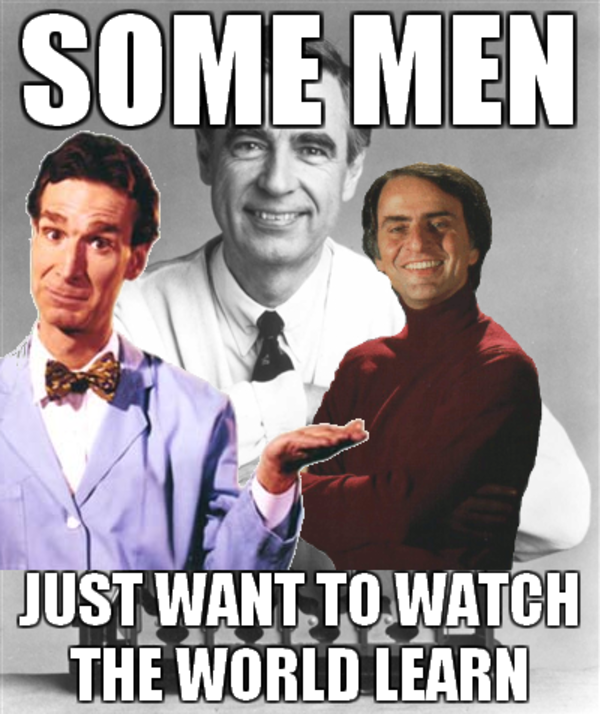
\includegraphics[width=0.4\textwidth]{images/watchandlearn.png}
\end{center}

\end{frame}

\begin{frame}
\frametitle{Remember the Initial Quiz}


Think back: what operations are fast and what operations are not?

Takeaway: our intuition  is often wrong. 

Not just at a macro level, but at a micro level. 

You may be able to narrow down that this computation of $x$ is slow, \\
but if you examine it carefully\ldots what parts of it are slow?


\end{frame}



\begin{frame}
\frametitle{Premature Optimization}

\vspace*{.5cm}

\begin{quote}
\textit{Programmers waste enormous amounts of time thinking about, or worrying about, the speed of noncritical parts of their programs, and these attempts at efficiency actually have a strong negative impact when debugging and maintenance are considered. We should forget about small efficiencies, say about 97\% of the time: premature optimization is the root of all evil. Yet we should not pass up our opportunities in that critical 3\%.}
\end{quote}
	\hfill -- Donald Knuth


\end{frame}



\begin{frame}
\frametitle{That Saying You Were Expecting}


Feeling lucky? \\
Maybe you optimized a slow part. 

\begin{center}
	
\includegraphics[width=0.4\textwidth]{images/feellucky.jpg}
\end{center}

To make your programs or systems fast, \\
you need to find out what is currently slow and improve it (duh!). 

Up until now, it's mostly been about \\
\qquad ``let's speed this up''.\\
We haven't taken much time to decide what we should speed up.

\end{frame}


\begin{frame}
\frametitle{Why Observation?}

\begin{center}
	
\includegraphics[width=0.5\textwidth]{images/observe.jpg}
\end{center}

Observation is a bit more than just measuring things.

\end{frame}


\begin{frame}
\frametitle{Kinds of Observation}

\begin{enumerate}
	\item Counters
	\item Profiles
	\item Traces
\end{enumerate}

We'll return to profiling later on.

\end{frame}


\begin{frame}
\frametitle{Tracing: Logging}

Logging is an effective way of finding out what's happening.

We have surely all used \texttt{printf} to debug!

Logs need: timestamp, message, \& attributes.

\end{frame}


\begin{frame}
\frametitle{Logging} 

If we get only one tool -- logging!

How often to log, and what content?

This may be our only shot to get that info...\\
\quad But don't drown out relevant things!


\end{frame}


\begin{frame}
\frametitle{Ideas}

Log input and output?

Want to be able to link things...


\end{frame}


\begin{frame}[fragile]
\frametitle{Example}

{\scriptsize
\begin{verbatim}
Received request: update plan of company 12345 to ULTIMATE
Retrieving company 12345
Verifying eligibility for upgrade of company 12345 from BASIC to ULTIMATE
Company 12345 is not eligible for upgrade due to: unpaid invoices > 0
Returning response: update of company 12345 to ULTIMATE is DECLINED
\end{verbatim}
}

\end{frame}


\begin{frame}
\frametitle{Timestamp Precision}

Timestamp precision depends on the timescale of execution.

Time zones matter. Recommendation: UTC!

Or Stardates?

\begin{center}
	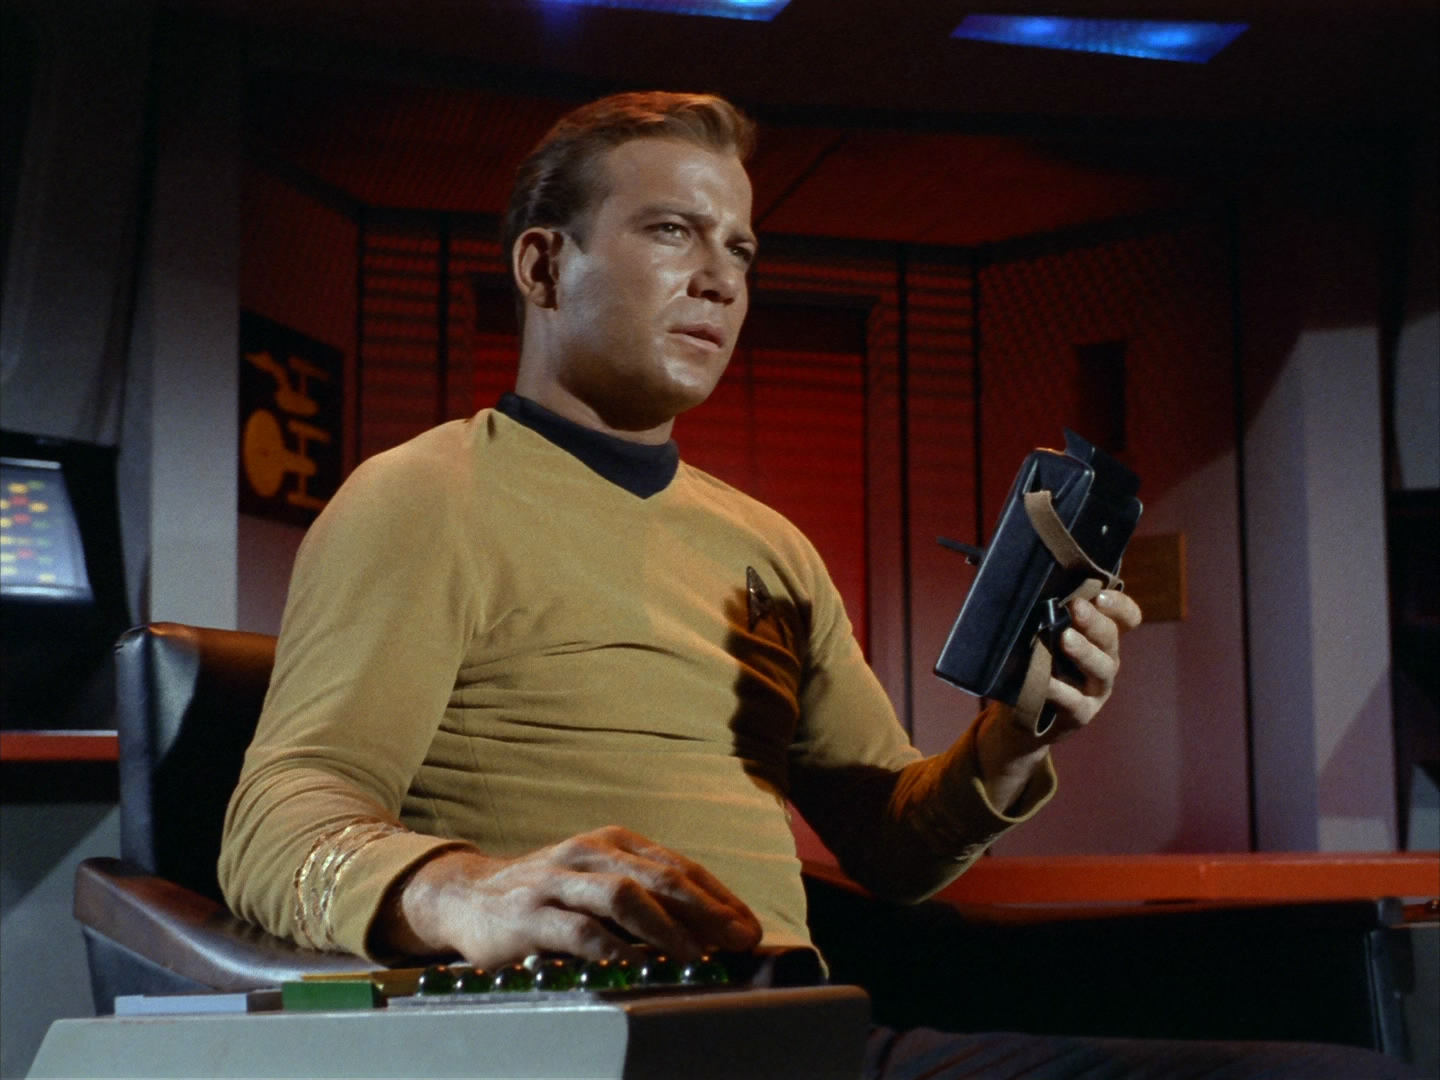
\includegraphics[width=0.4\textwidth]{images/captainslog.jpg}
\end{center}

\end{frame}


\begin{frame}
\frametitle{Too Much Noise}

Logging every request might be too noisy.

Searching and sorting help!

Too much detail is also bad...

\end{frame}


\begin{frame}
\frametitle{Personally Identifiable Information = No}

\begin{center}
	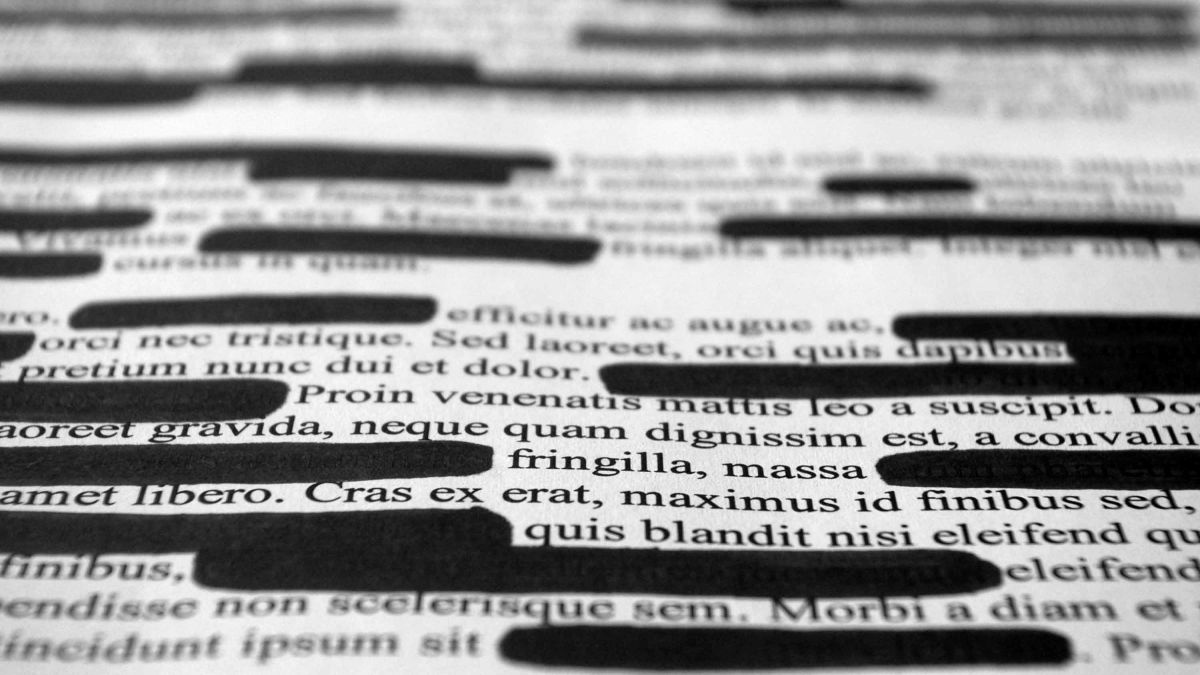
\includegraphics[width=\textwidth]{images/redacted.jpg}
\end{center}

\end{frame}


\begin{frame}
\frametitle{Over-logging}

Is it too hard to get access to info other ways?

Aim for a balance.


\end{frame}


\begin{frame}
\frametitle{Overhead of Tracing}

CPU trace tool: $20\times$ slowdown.

Timestamp at function call: $1.2-1.5\times$ slowdown.

Timestamp of system call entry/exit: $< 1\%$

\end{frame}


\begin{frame}
\frametitle{Other Overhead Tracing}

Valgrind: Up to $100\times$ slowdown.

Disk trace: pretty minimal!

Can identify deadlocks and waiting for locks.

\end{frame}


\begin{frame}
\frametitle{Space, the Final Frontier}

\begin{center}
	
\includegraphics[width=0.3\textwidth]{images/finalfrontier.jpg}
\end{center}
\hfill Image Credit: Revma Mahita

The trace itself takes up space.

20 GB/s bandwidth and 64-byte cache lines recording up to 8 bytes of data per trace entry could result in producing data at a rate of 2.4 GB per second.

\end{frame}


\begin{frame}
\frametitle{Counters}

Counters, as the name suggests, keep a count of events: interrupts, cache misses, data bytes written, calls to function \texttt{do\_magic()}.


Counters are aggregation, because we're summing the number of occurrences.

\end{frame}


\begin{frame}
\frametitle{Other Aggregation}

Average response time is aggregation: total time and number of requests.

Asking the computer to calculate the summary is sensible.

Ideas: number of requests, requests broken down by type, average time to respond to a request, percentage of error responses...  


\end{frame}


\begin{frame}
\frametitle{Context is Key}

\begin{center}
	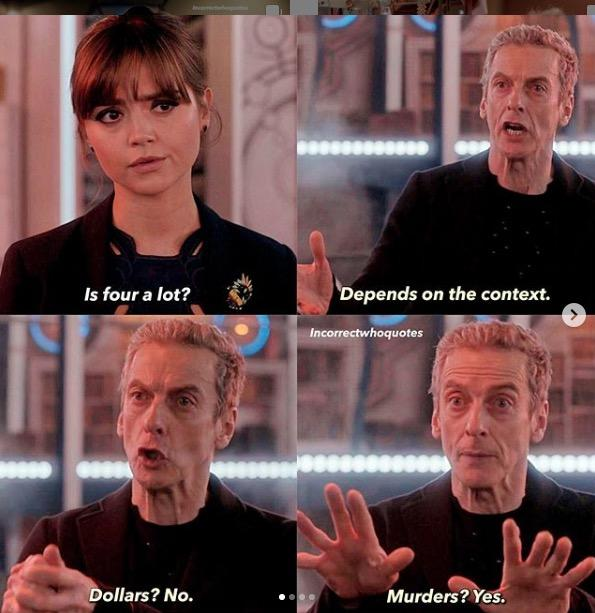
\includegraphics[width=0.6\textwidth]{images/context.jpg}
\end{center}


\end{frame}


\begin{frame}
\frametitle{Context to Aggregation}

After my PR, login time $0.75s$ -- Good or bad?

Depends on the baseline. Maybe it was $0.5s$?


Okay, increased -- is that bad?

\end{frame}


\begin{frame}
\frametitle{Another Example}

Request takes on average $1.27s$ -- Good or Bad?

What if the time limit is 1 second? 10 seconds?

How hard is the deadline?

\end{frame}


\begin{frame}
\frametitle{Averages Misleading}

All of these are 7 requests per second on average:

\begin{center}
	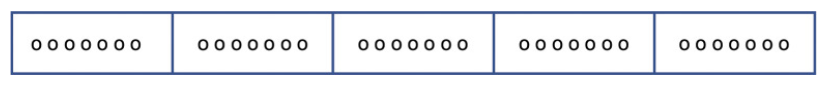
\includegraphics[width=\textwidth]{images/burst1}\\
	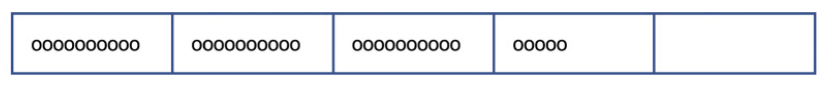
\includegraphics[width=\textwidth]{images/burst2}\\
	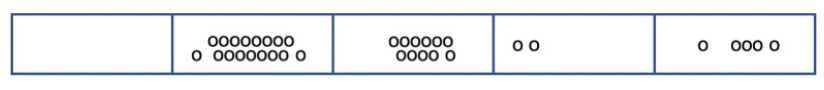
\includegraphics[width=\textwidth]{images/burst3}\\
\end{center}


\end{frame}

\begin{frame}
\frametitle{Time Period}

When we aggregate, we have to choose the period of time.

Whole execution of the task?

Indefinitely-running services?

We might miss important things!

\end{frame}


\begin{frame}
\frametitle{Look at the Pretty Pictures}

Graphs and visualizations help us see trends in data.

\begin{center}
	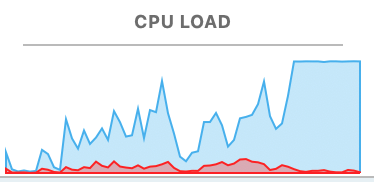
\includegraphics[width=0.7\textwidth]{images/cpu-load.png}
\end{center}

Managers and non-techies love them!

If we put together enough pretty pictures, we get a dashboard.

\end{frame}


\begin{frame}
\frametitle{Dashboards}

Dashboards are ideally more than just pretty pictures of LINE GOES UP.

\begin{center}
	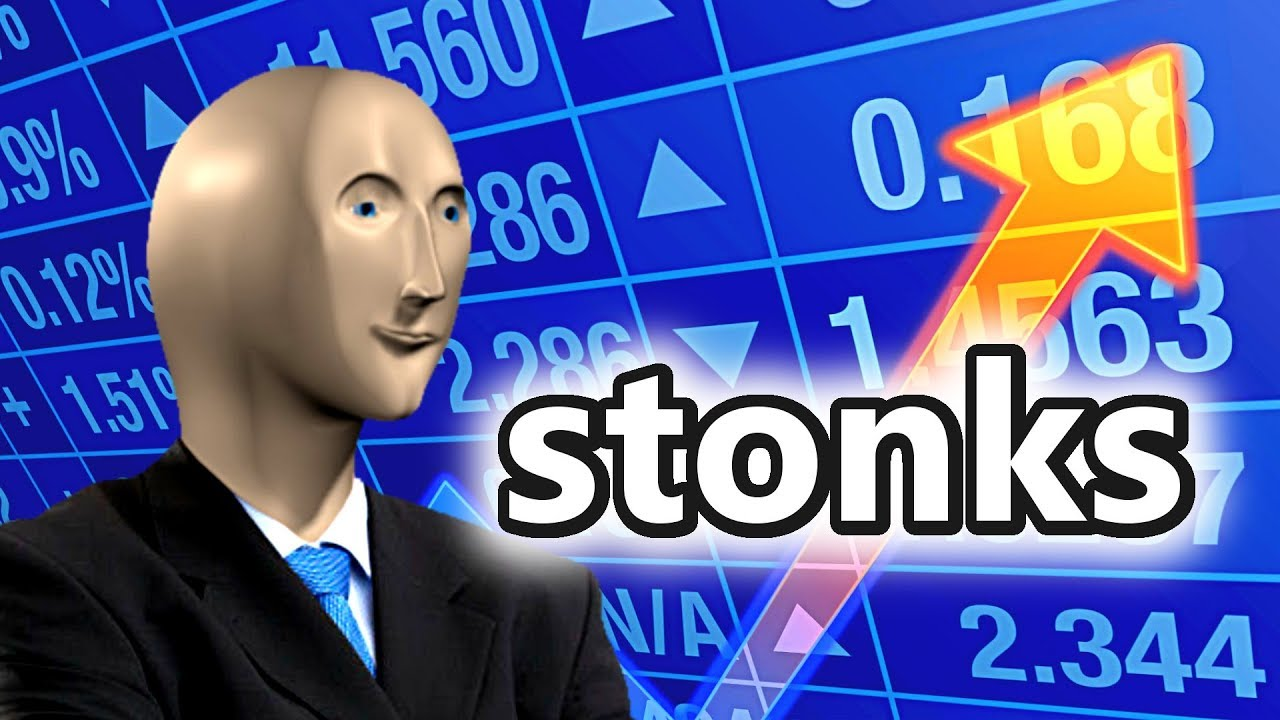
\includegraphics[width=\textwidth]{images/stonks.jpg}
\end{center}

Should present an easily-digestible summary.

\end{frame}


\begin{frame}
\frametitle{Drill Down}

This is just a high level idea of identifying what's happening.

As we proceed we need to get to lower level tools.

Next: narrowing down where the bottleneck is.

\end{frame}






\end{document}

